\documentclass[problem]{mcs}

\begin{pcomments}
  \pcomment{from: S09.cp7t}
  \pcomment{from: S07.cp6f}
  \pcomment{There is a lot of commented out material regarding 2k-cycle networks.  We had a final exam problem on them that might be nice to include along with the 2k-cycleproblem as a challenge problem.}
\end{pcomments}

\pkeywords{
  networks
}

%%%%%%%%%%%%%%%%%%%%%%%%%%%%%%%%%%%%%%%%%%%%%%%%%%%%%%%%%%%%%%%%%%%%%
% Problem starts here
%%%%%%%%%%%%%%%%%%%%%%%%%%%%%%%%%%%%%%%%%%%%%%%%%%%%%%%%%%%%%%%%%%%%%

\begin{problem}
A \emph{5-path} communication network is shown below.  From this, it's
easy to see what an $n$-path network would be.  Fill in the table of
properties below, and be prepared to justify your answers.

\begin{center}
\begin{tabular}{ccc}
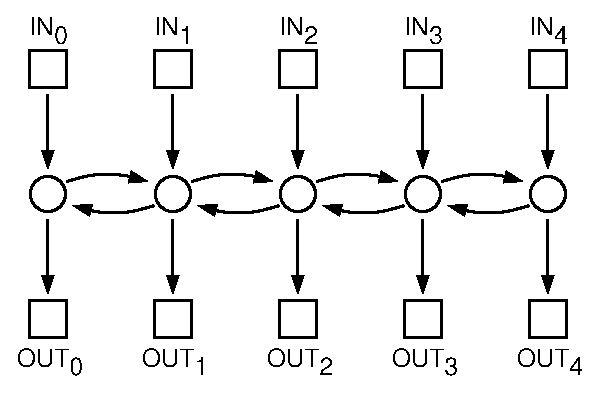
\includegraphics[height=1.5in]{figures/line-nw}\\
% & & 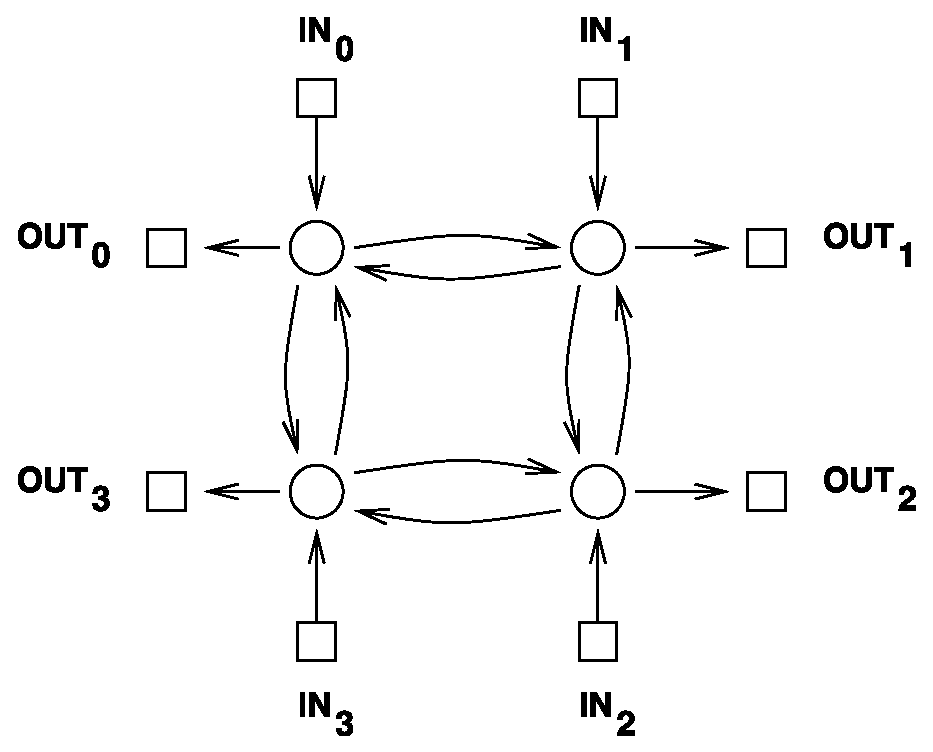
\includegraphics[height=2in]{figures/cycle4} \\
\textbf{5-Path}% & \qquad & \textbf{4-Cycle}
\end{tabular}
\end{center}

{\large
\[
\begin{array}{c|c|c|c|c}
\text{network} &
\text{\# switches} &
\text{switch size} &
\text{diameter} &
\text{max congestion} \\ \hline
\text{5-path} &
\insolutions{5} &
\insolutions{3 \times 3} &
\insolutions{6} &
\insolutions{5} \\ \hline
\text{$n$-path} &
\insolutions{n} &
\insolutions{3 \times 3} &
\insolutions{n+1} &
\insolutions{n}
\end{array}
\]
}

\solution{The congestion of the $n$-path is at least $n$, because every
path must contain the central switch when $\pi(i) = n- 1 - i$.  The congestion
is at most $n$, because there are only $n$ simple paths in total.  The longest
path is from input 0 to output $n-1$ of length $n+1$, so this is the
diameter.}

\iffalse
The congestion of the 4-cycle is at least 3.  Consider the permutation
routing problem in which each input sends a packet to the diagonally
opposite output: $\pi(0) = 2$, $\pi(1) = 3$, $\pi(2) = 0$, $\pi(3) =
1$.  Packets 0 and 2 must pass through the switches on the upper left
and lower right in order to access the appropriate input and output
terminals.  Packets 1 must pass through one of these switches as well,
so at least three packets pass through either the upper-left switch or
the lower-left switch.

The congestion of the 4-cycle is at most 3.  Suppose we route each
packet by the shortest path and break ties by routing clockwise around
the cycle.  Now consider any particular switch, say the one in the
upper right.  At worst, this switch sees three packets: the one from
input 1, the one destined for output 1, and one passing through from
input 0 to output 2.  By symmetry, every switch sees at most 3 packets.}
\fi

\iffalse

\ppart Now consider the $n$-path and $2k$-cycle networks, and again fill in the
table below. (The $2k$-cycle is a $k \times k$ rectangular arrangement
with $k$ inputs on the top and bottom sides of the rectangle, and $k$
outputs on the left and right sides.)


{\large
\[
\begin{array}{c|c|c|c|c}
\text{network} &
\text{\# switches} &
\text{switch size} &
\text{diameter} &
\text{max congestion} \\ \hline
\text{$n$-path} &
\insolutions{n} &
\insolutions{3 \times 3} &
\insolutions{n+1} &
\insolutions{n} \\ \hline
\text{$2k$-cycle} &
\insolutions{4(k-1)} &
\insolutions{ 3 \times 3, 2\times 3, 3 \times 2 } &
\insolutions{2(k-1)+2 = 2k} &
\insolutions{k+1}
\end{array}
\]
}

\solution{TBA

\mfigure{!}{3in}{figures/2kCycle}
}

\eparts
\fi

\end{problem}

%%%%%%%%%%%%%%%%%%%%%%%%%%%%%%%%%%%%%%%%%%%%%%%%%%%%%%%%%%%%%%%%%%%%%
% Problem ends here
%%%%%%%%%%%%%%%%%%%%%%%%%%%%%%%%%%%%%%%%%%%%%%%%%%%%%%%%%%%%%%%%%%%%%
